\documentclass[9pt, aspectratio=169, handout]{beamer}

% +==================================================+
% |   ████████╗██╗  ██╗███████╗███╗   ███╗███████╗   |
% |   ╚══██╔══╝██║  ██║██╔════╝████╗ ████║██╔════╝   |
% |      ██║   ███████║█████╗  ██╔████╔██║█████╗     |
% |      ██║   ██╔══██║██╔══╝  ██║╚██╔╝██║██╔══╝     |
% |      ██║   ██║  ██║███████╗██║ ╚═╝ ██║███████╗   |
% |      ╚═╝   ╚═╝  ╚═╝╚══════╝╚═╝     ╚═╝╚══════╝   |
% +==================================================+

\useinnertheme{rectangles}
\useoutertheme{infolines}

\setbeamertemplate{footline}{%
    \leavevmode%
    \rule{\paperwidth}{0.1pt}\vskip0.2pt%
    \hbox{%
        \begin{beamercolorbox}[wd=.2\paperwidth, ht=2.25ex, dp=1ex, center]{author in head/foot}%
            \usebeamerfont{author in head/foot}\insertshortauthor
        \end{beamercolorbox}%
        \begin{beamercolorbox}[wd=.6\paperwidth, ht=2.25ex, dp=1ex, center]{title in head/foot}%
            \usebeamerfont{title in head/foot}\insertshorttitle
        \end{beamercolorbox}%
        \begin{beamercolorbox}[wd=.2\paperwidth, ht=2.25ex, dp=1ex, center]{date in head/foot}%
            \usebeamerfont{date in head/foot}\insertshortdate\hfill\insertframenumber{} / \inserttotalframenumber\hspace*{2ex}
        \end{beamercolorbox}%
    }%
    \vskip0pt%
}
% hrule under the frametitle, see:
% https://tex.stackexchange.com/questions/343517/beamer-full-width-hrule-below-frame-title
\setbeamertemplate{frametitle}{%
    \usebeamerfont{frametitle}\insertframetitle%
    \vphantom{g}%
    \par%
    \makebox[\linewidth][c]{%
        \rule[0.5\baselineskip]{\paperwidth}{0.4pt}%
    }%
}

% \beamertemplatenavigationsymbolsempty % remove navigation bar

\definecolor{grey80}{HTML}{CCCCCC}
\definecolor{grey90}{HTML}{E6E6E6}
\definecolor{grey95}{HTML}{F2F2F2}

\usepackage[svgnames, x11names]{xcolor}
\usecolortheme[named=DarkSlateGrey]{structure}
\setbeamercolor{background canvas}{bg=white}

\setbeamerfont{frametitle}{series=\bfseries}

\let\oldtiny\tiny
\let\oldscriptsize\scriptsize
\let\oldfootnotesize\footnotesize
\let\oldsmall\small
\let\oldnormalsize\normalsize
\let\oldlarge\large
\let\oldLarge\Large
\let\oldLARGE\LARGE
\let\oldhuge\huge
\let\oldHuge\Huge
\renewcommand*{\footnotesize}{\oldfootnotesize\scriptsize}
\renewcommand*{\normalsize}{\oldnormalsize\oldsmall}
\setbeamerfont{frametitle}{size=\oldnormalsize}

% +=================================+
% |   ██████╗ ██╗██████╗ ███████╗   |
% |   ██╔══██╗██║██╔══██╗██╔════╝   |
% |   ██████╔╝██║██████╔╝███████╗   |
% |   ██╔══██╗██║██╔══██╗╚════██║   |
% |   ██████╔╝██║██████╔╝███████║   |
% |   ╚═════╝ ╚═╝╚═════╝ ╚══════╝   |
% +=================================+

% \usepackage[style=nejm,backend=biber]{biblatex}
% \addbibresource{my.bib}
% \renewcommand*{\bibfont}{\footnotesize}

% +==========================================+
% |   ███╗   ███╗ █████╗ ████████╗██╗  ██╗   |
% |   ████╗ ████║██╔══██╗╚══██╔══╝██║  ██║   |
% |   ██╔████╔██║███████║   ██║   ███████║   |
% |   ██║╚██╔╝██║██╔══██║   ██║   ██╔══██║   |
% |   ██║ ╚═╝ ██║██║  ██║   ██║   ██║  ██║   |
% |   ╚═╝     ╚═╝╚═╝  ╚═╝   ╚═╝   ╚═╝  ╚═╝   |
% +==========================================+

\usepackage{amsmath,amssymb,amsfonts}
\usepackage{cancel}
\usepackage{braket}
\usepackage{bm}
\usepackage{siunitx}
\usepackage{feynmf}
\usepackage{cleveref}
\DeclareGraphicsRule{*}{mps}{*}{}

% +===================================================+
% |   ███████╗██╗ ██████╗ ██╗   ██╗██████╗ ███████╗   |
% |   ██╔════╝██║██╔════╝ ██║   ██║██╔══██╗██╔════╝   |
% |   █████╗  ██║██║  ███╗██║   ██║██████╔╝█████╗     |
% |   ██╔══╝  ██║██║   ██║██║   ██║██╔══██╗██╔══╝     |
% |   ██║     ██║╚██████╔╝╚██████╔╝██║  ██║███████╗   |
% |   ╚═╝     ╚═╝ ╚═════╝  ╚═════╝ ╚═╝  ╚═╝╚══════╝   |
% +===================================================+
\usepackage{subcaption}
\usepackage{makecell}
\usepackage{booktabs}

% +===========================================================+
% |    ██████╗██╗  ██╗██╗███╗   ██╗███████╗███████╗███████╗   |
% |   ██╔════╝██║  ██║██║████╗  ██║██╔════╝██╔════╝██╔════╝   |
% |   ██║     ███████║██║██╔██╗ ██║█████╗  ███████╗█████╗     |
% |   ██║     ██╔══██║██║██║╚██╗██║██╔══╝  ╚════██║██╔══╝     |
% |   ╚██████╗██║  ██║██║██║ ╚████║███████╗███████║███████╗   |
% |    ╚═════╝╚═╝  ╚═╝╚═╝╚═╝  ╚═══╝╚══════╝╚══════╝╚══════╝   |
% +===========================================================+

% \usepackage{xeCJK}
% \setCJKmainfont{PingFang SC}

% +====================================+
% |   ███╗   ███╗██╗███████╗ ██████╗   |
% |   ████╗ ████║██║██╔════╝██╔════╝   |
% |   ██╔████╔██║██║███████╗██║        |
% |   ██║╚██╔╝██║██║╚════██║██║        |
% |   ██║ ╚═╝ ██║██║███████║╚██████╗   |
% |   ╚═╝     ╚═╝╚═╝╚══════╝ ╚═════╝   |
% +====================================+

\usepackage{fontawesome5}
\usepackage{twemojis}
\newcommand{\myhl}[1]{\textcolor{DeepPink}{#1}}
\newcommand{\myhlb}[1]{\textcolor{Blue}{#1}}


\title{MAE 131A Discussion Sections\\ Week 7}
\author{Matthew Taliaferro}
\institute[UCLA MAE]{Mechanical and Aerospace Engineering Department\\
    University of California, Los Angeles}
\date{Nov 15, 2024}

\begin{document}

\begin{frame}
    \titlepage
\end{frame}

\begin{frame}{Problem 1 (11.20 in the book)}
    \textbf{Problem 11.20}.
        Consider a concentric tube heat exchanger with an area of \SI{50}{\square\meter} operating under the following conditions:

    \begin{center}
        \begin{tabular}{lcc}
            \toprule
            ~ & Hot Fluid & Cold Fluid \\
            \midrule
            Heat capacity rate, \si{\kilo\watt\per\kelvin} & 6 & 3 \\
            Inlet temperature, \si{\celsius} & 60 & 30 \\
            Outlet temperature, \si{\celsius} & ? & 54 \\
            \bottomrule
        \end{tabular}
    \end{center}

    
    \begin{enumerate}
        \item Determine the outlet temperature of the hot fluid.
        \item Is the heat exchanger operating in counterflow or parallel flow, or can't you tell from the available information?
        \item Calculate the overall heat transfer coefficient.
        \item Calculate the effectiveness of this exchanger.
        \item What would be the effectiveness of this exchanger if its length were made very large?
    \end{enumerate}
\end{frame}

\begin{frame}[allowframebreaks]{Problem 1 Solution}
    \begin{enumerate}
        \item The energy transferred from one fluid is absorbed by the other.

        \begin{gather*}
            q = C_c \left( T_{c,o} - T_{c,i} \right) \\
            q = C_h \left( T_{h,i} - T_{h,o} \right) \\ 
            \to C_c \left( T_{c,o} - T_{c,i} \right) = C_h \left( T_{h,i} - T_{h,o} \right) \\
            \to T_{h,o} = \SI{48}{\celsius}
        \end{gather*}

        \item The outlet temperature for the ``hot'' fluid is lower than the outlet temperature for the ``cold'' fluid.
            Has to be counterflow.
        \item The expression for the logarithmic mean temperature methodology is:

            \begin{equation*}
                q = \mathit{UA} \Delta T_{lm},
            \end{equation*}

            where

            \begin{equation*}
                \Delta T_{lm} = \frac{\Delta T_1 - \Delta T_2}{\mathrm{ln} \left( \frac{\Delta T_1}{\Delta T_2} \right)} = \SI{10.9}{\celsius}.
            \end{equation*}

            We have the overall heat transfer from the first part, so we just need to rearrange the equation.

            \begin{equation*}
                \mathit{UA} = \frac{q}{\Delta T_{lm}} \to \mathit{UA} = \SI{132}{\watt\per\square\meter\per\kelvin}
            \end{equation*}
        \item Using the definition of the effectiveness:
            \begin{equation*}
                \epsilon = \frac{q}{q_{\mathit{max}}} = \frac{C_c \left( T_{c,o} - T_{c,i}  \right)}{C_{\mathit{min}} \left( T_{h,i} - T_{c,o}  \right)} = 0.8
            \end{equation*}
        \item For a very long heat exchanger, almost all the heat transfer that can be transferred will be transferred.
            \begin{equation*}
                \epsilon = \frac{q}{q_{\mathit{max}}} = 1
            \end{equation*}
    \end{enumerate}
\end{frame}




\begin{frame}{Problem 2 (11.58 in the book)}
    \textbf{Problem 11.58}.
        A shell-and-tube heat exchanger with one shell pass and 20 tube passes uses hot water on the tube side to heat oil on the shell side.
        The single copper tube has inner and outer diameters of 20 and 24 \si{\milli\meter} and a length per pass of \SI{3}{m}.
        The water enters at \SI{87}{\celsius} and 0.2 kg/s and leaves at \SI{27}{\celsius}.
        Inlet and outlet temperatures of the oil are \SI{7}{\celsius} and \SI{37}{\celsius}.
        What is the average convection coefficient for the tube outer surface?

    \vspace{1ex}
    \textbf{Exploratory:}
        If using the logarithmic mean temperature method, what correction factor would be needed to make it work?
        Estimate the Reynolds number of the oil.
\end{frame}

\begin{frame}{Problem 2 Relevent Equations}
    \begin{columns}
        \begin{column}{0.25\textwidth}
            \begin{figure}
                \begin{center}
                    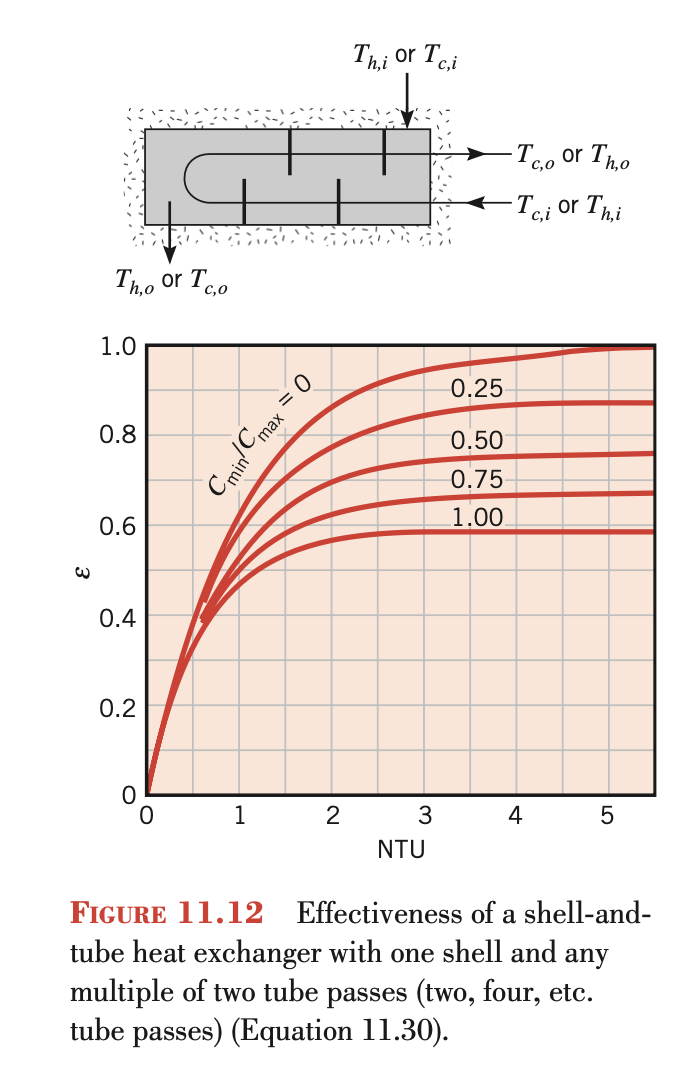
\includegraphics[width=0.95\textwidth]{Figures/fig7.1.png}
                \end{center}
            \end{figure}
        \end{column}
        

        \begin{column}{0.75\textwidth}
            \begin{figure}
                \begin{center}
                    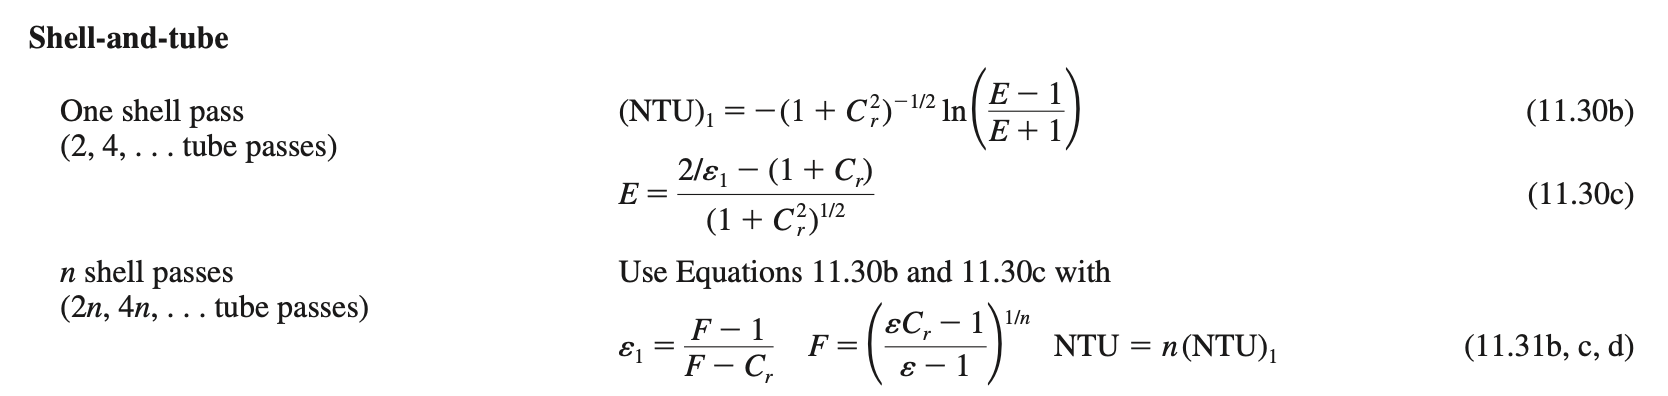
\includegraphics[width=0.95\textwidth]{Figures/fig7.2.png}
                    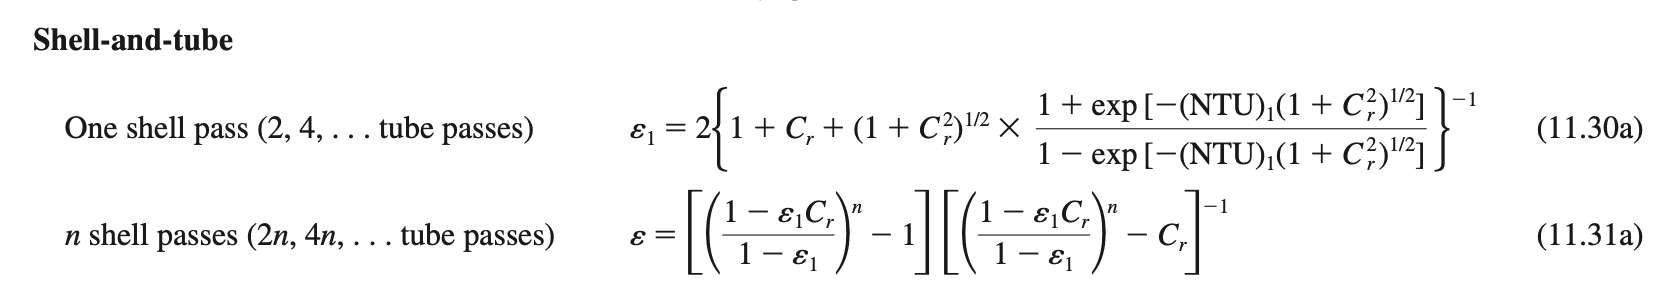
\includegraphics[width=0.95\textwidth]{Figures/fig7.3.png}
                \end{center}
            \end{figure}
        \end{column}
    \end{columns}
\end{frame}

\begin{frame}[allowframebreaks]{Problem 2 Solution}
    \begin{itemize}
        \item We can find the overall heat transfer coefficient fairly easily using the effectiveness-NTU method.
            
            \begin{gather*}
                \epsilon = \frac{q}{q_{\mathrm{max}}} = 0.75 \\
                \mathit{NTU} = 1 \left( 1 + C_r^2 \right)^{-1/2} \mathrm{ln} \left( \frac{E - 1}{E + 1} \right) = 3.44 \\
                E = \frac{2/\epsilon - \left( 1 + C_r \right)}{\left( 1 + C_r \right)^{1/2}} = 1.04 \\
            \end{gather*}

        \item We are asked to find the \textbf{average} heat transfer coefficient on the outer surface.
            From $\mathit{NTU}$ we can find the overall heat transfer coefficient, $\mathit{UA}$, which we can use to find one component of $\mathit{UA}$.
            
            \begin{equation*}
                \frac{1}{\mathit{UA}} = \frac{1}{h_i A_i} + \frac{1}{h_o A_o}
            \end{equation*}
            
            Why can use this equation?
        \item Given the constraints of the problem, the easiest way is to find $h_i$.
            \begin{gather*}
                \mathit{Nu}_D = f \left( \mathit{Re}_D, \mathit{Pr}_D \right) \\
                \mathit{Re}_D \approx \frac{4 \dot{m}}{\pi D_i \mu} = \num{2.6 e 4} \\
                \mathit{Pr}_D = 3.15 \\
                \mathit{Nu}_D = \frac{\left( f/8 \right) \left( \mathit{Re}_D - 1000 \right) \mathit{Pr}}{1 + 12.7 \sqrt{f/8} \left( \mathit{Pr}^{2/3} - 1 \right)} = 133.6
            \end{gather*}

            Note, the Dittus-Boelter equation gives $\mathit{Nu}_D = 110.8$.

            Rearranging the expression for $\mathit{UA}$ gives the heat transfer coefficient on the outside:
            
            \begin{equation*}
                h_o = \SI{773}{\watt\per\square\meter\per\kelvin}
            \end{equation*}

            Note, the Dittus-Boelter equation gives $h_o = \SI{809}{\watt\per\square\meter\per\kelvin}$.
    \end{itemize}
\end{frame}

\end{document}
